\begin{frame}
    \frametitle{\problemtitle}
    \begin{block}{Problem}
        Given an integer $s$, output the minimum radius of a circle that contains $> s$ whole unit squares.
    \end{block}

    \pause
    \begin{center}
        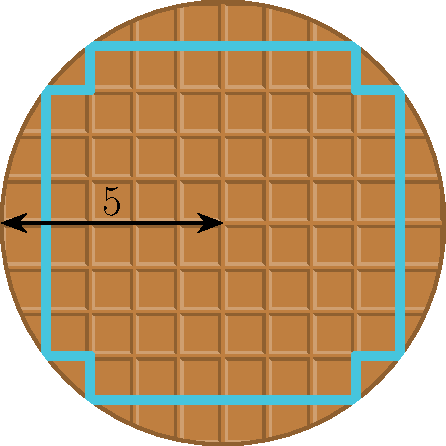
\includegraphics[height=0.35\textheight]{sample}
    \end{center}

    \pause
    \begin{block}{Solution}
        \begin{itemize}
            \item<+-> For a fixed radius $r$, we can determine the number of whole unit squares that fit in the circle.
            \item<+-> Determine how many squares fit in each column using
                the Pythagorean Theorem. ($\mathcal O(\sqrt s)$)
            \item<+-> Use binary search to find the solution. Total time:
                $\mathcal O(\log s \cdot \sqrt s)$.
        \end{itemize}
    \end{block}
\end{frame}
\begin{frame}
    \frametitle{\problemtitle}
    \begin{block}{Problem}
        Given an integer $s$, output the minimum radius of a circle that contains $> s$ whole unit squares.
    \end{block}

    \begin{center}
        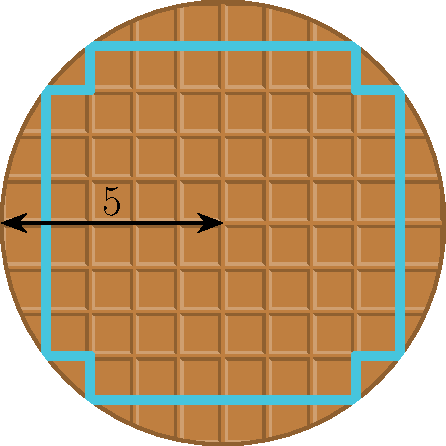
\includegraphics[height=0.35\textheight]{sample}
    \end{center}

    \begin{block}{Challenge}
        It is possible in $\mathcal O(\sqrt s)$ as well.
    \end{block}
    \pause
    \solvestats
\end{frame}
